\chapter{Background}

\section{Large language models}
Large language models (LLMs) lie at the core of the current AI revolution. They are parametric probabilistic models that learn to represent the distribution of natural language sequences and generate text by autoregressively predicting one token at a time. Formally, given a tokenized sequence $(x_1, \dots, x_T)$, an LLM models $p(x_{1:T})=\prod_{t=1}^T p(x_t \mid x_{<t})$ and is trained to minimize the cross-entropy between predicted and observed tokens. LLMs derive their broad linguistic and factual knowledge from pretraining on massive text corpora using this objective, which at scale enables emergent capabilities such as in-context learning and reasoning.

\subsection{Objective and pretraining}
The standard objective is a next-token prediction:
\begin{equation}
\mathcal{L}(\theta) = - \sum_{t=1}^{T} \log p_\theta(x_t \mid x_{<t}),
\end{equation}
optimized over large, diverse datasets using gradient descent. Conceptually, this process can be understood as a vast, GPU-driven lossy compression - the model distills the statistical regularities and patterns of human language into a compact, parameterized form that enables general-purpose text understanding and generation. While pretraining is purely self-supervised, downstream adaptation may use supervised fine-tuning or preference-based methods to align behavior.

\subsection{Transformer}
Transformer architecture \cite{vaswani2023attentionneed} underlies most modern LLMs. The main building blocks are:

\begin{itemize}
    \item \textbf{Embeddings and positional encoding}: Tokens are mapped to dense vectors and augmented with position information, either sinusoidal or learned, to make the model order-aware.
    \item \textbf{Multi-head self-attention}: For each position, queries $Q$, keys $K$, and values $V$ are computed by linear projections of the hidden states. Scaled dot-product attention aggregates information across positions:
    \begin{equation}
    \mathrm{Attn}(Q,K,V) = \mathrm{softmax}\!\left(\frac{QK^{\top}}{\sqrt{d_k}}\right) V.
    \end{equation}
    Multiple heads attend in parallel to different subspaces, and their outputs are concatenated and projected.
    \item \textbf{Position-wise feed-forward network (FFN)}: A two-layer MLP with a nonlinearity (e.g., GELU) is applied independently to each position.
    \item \textbf{Residual connections and layer normalization}: Each sublayer is wrapped with residual additions and normalization for stability.
\end{itemize}

Computationally, attention has $O(L^2 d)$ time and $O(L^2)$ memory in sequence length $L$ (per batch and head factors omitted), while FFNs dominate parameter count with $O(d^2)$.

\begin{figure}[!h]
    \centering
    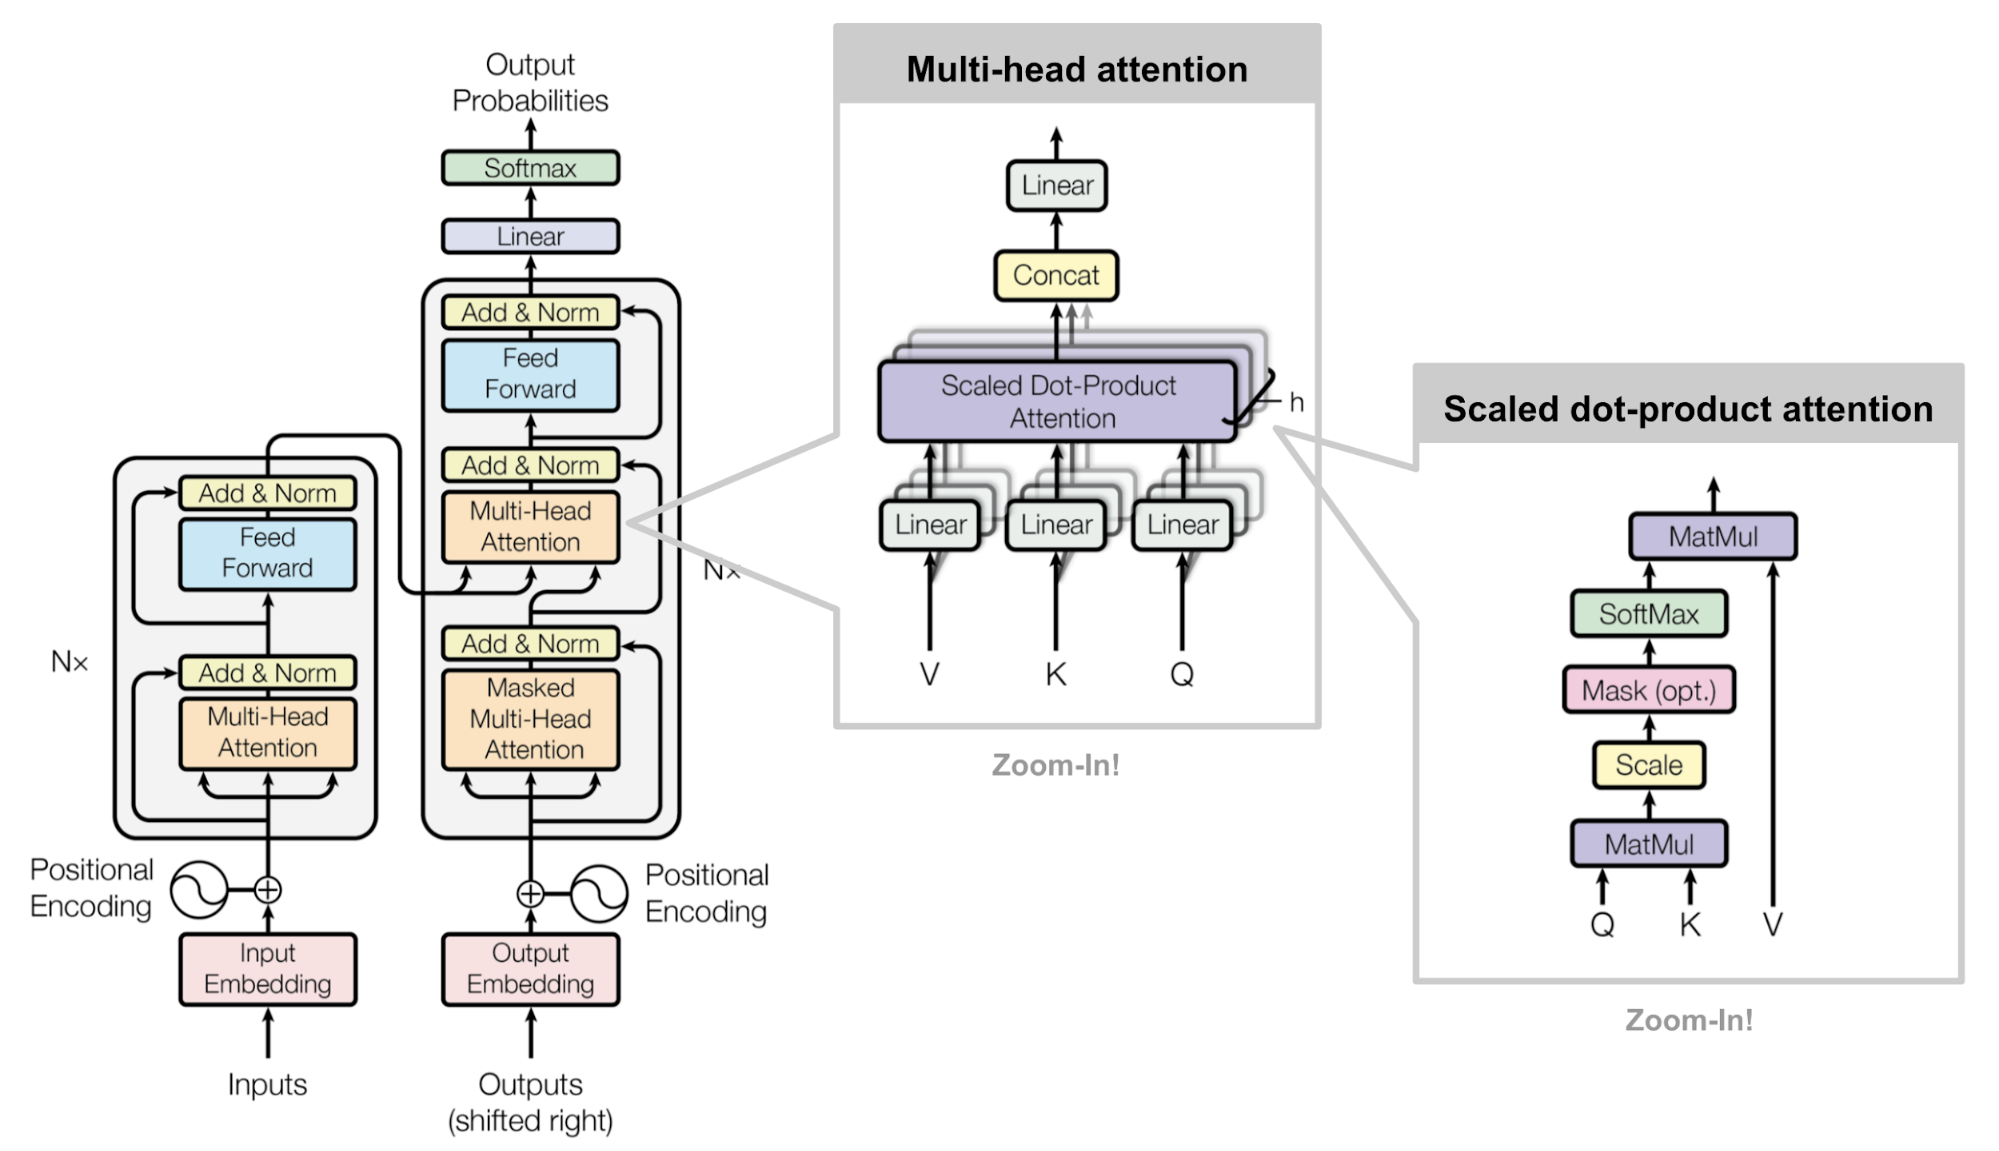
\includegraphics[width=\linewidth]{img/transformer.png}
    \caption{Transformer encoder-decoder block}
    \label{fig:transformer-block}
\end{figure}

\subsection{Decoder-only LLMs}
Decoder-only LMs use a lower-triangular mask in self-attention so that token $t$ attends only to positions $< t$. This enforces autoregressive factorization and enables left-to-right generation. During inference, key-value (KV) caching stores past projections to avoid recomputation, reducing per-token latency from quadratic to approximately linear in $L$ for attention, with constant-depth projections per layer.

\subsection{Scaling laws}
Transformers scale predictably with model size (parameters), data (tokens), and compute. Empirically, test loss follows power-law scaling with these resources \cite{kaplan2020scalinglawsneurallanguage}, implying steady gains as capacity and data increase. Practical costs rise superlinearly with size due to:

\begin{itemize}
    \item \textbf{Training}: attention's $O(L^2)$ complexity amplifies FLOPs and memory.
    \item \textbf{Inference}: latency and memory scale with depth and width; context length increases multiply attention cost without specialized kernels.
\end{itemize}

Despite costs, scaling yields emergent capabilities such as in-context learning and improved generalization \cite{brown2020languagemodelsfewshotlearners}.

\begin{figure}[!h]
    \centering
    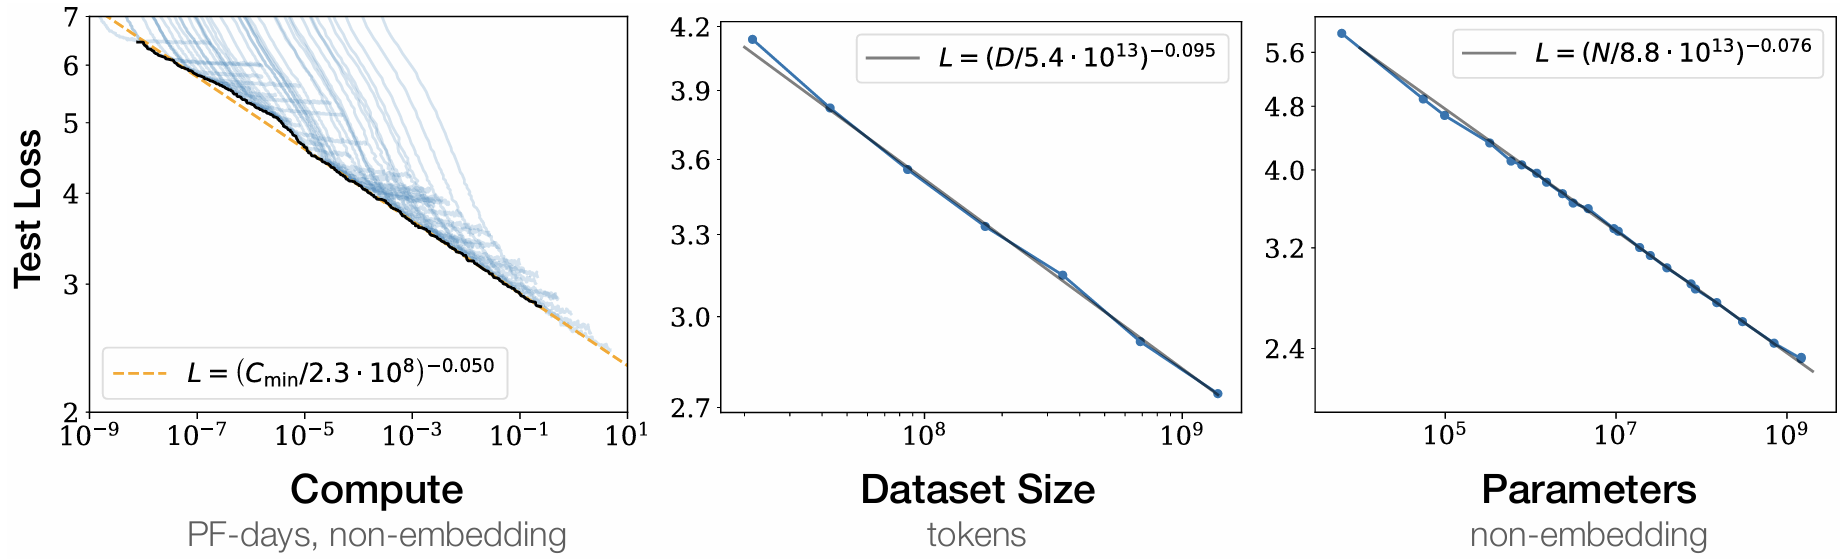
\includegraphics[width=\linewidth]{img/scaling_laws.png}
    \caption{Scaling laws: test loss vs. effective compute/model size/data on logarithmic axes.}
    \label{fig:scaling-laws}
\end{figure}

\subsection{Limitations and small-model challenges}
Large language models are known to have several limitations including:

\begin{itemize}
    \item \textbf{Hallucinations}: the model may produce fluent but unsupported statements.
    \item \textbf{Context and computation limits}: finite context windows and lack of external working memory hinder long-horizon tasks.
    \item \textbf{Compositionality}: chaining steps and maintaining intermediate variables is difficult under greedy decoding.
\end{itemize}

Small models (e.g., <4B parameters) face additional constraints which degrade multi-step arithmetic and logical reasoning, especially when strict output formats are required. While prompting and decoding strategies can mitigate some issues, structural capacity often remains the bottleneck without additional supervision or architectural support.

\section{Prompting}
Prompting is a practice of specifying a model's task through natural language. It functions as a programming interface to language models. Instruction tuning and alignment methods improve adherence to prompts \cite{ouyang2022traininglanguagemodelsfollow}.

\subsection{Paradigms}
Several prompting paradigms have emerged, often combined in practice:
\begin{itemize}
    \item \textbf{Zero-shot prompting}: The model receives only task instructions and the input. This tests inherent generalization from pretraining and any instruction tuning. It is simple and cheap but sensitive to wording and often weaker on tasks requiring intermediate computation.
    \item \textbf{Few-shot prompting}: The prompt includes $k$ input-output examples that implicitly define the task and desired format, enabling in-context learning \cite{brown2020languagemodelsfewshotlearners}.
    \item \textbf{Chain-of-Thought (CoT) prompting}: The prompt requests step-by-step reasoning, eliciting intermediate rationales before the final answer \cite{wei2023chainofthoughtpromptingelicitsreasoning}. CoT can improve complex, multi-step tasks like arithmetic by encouraging deliberate decomposition, but increases latency and token usage.
\end{itemize}

\section{Knowledge distillation}
Knowledge distillation (KD) transfers the behavior of a high-capacity teacher model to a typically smaller student \cite{hinton2015distilling}. The core idea is that softened target distributions carry "dark knowledge" about class or token similarities that hard labels do not expose, often improving generalization while enabling compression and faster inference.

\subsection{Objectives and loss design}
Response-based KD is the most widely used approach. In this setting, the student is trained to match the teacher's output distribution. Let $z^{(T)}$ and $z^{(S)}$ be teacher and student logits, and $T>0$ a temperature. The softened distributions are $p^{(T)}=\mathrm{softmax}(z^{(T)}/T)$ and $p^{(S)}=\mathrm{softmax}(z^{(S)}/T)$. A common loss combines distillation with standard supervision:
\begin{equation}
\mathcal{L} = (1-\alpha)\,\mathrm{CE}(y,\ \mathrm{softmax}(z^{(S)})) + \alpha\, T^2\, \mathrm{KL}\!\left(p^{(T)} \,\|\, p^{(S)}\right),
\end{equation}
where $y$ are hard labels and $\alpha \in [0,1]$ balances terms; the $T^2$ factor compensates for gradient scaling \cite{hinton2015distilling}.

Beyond responses, feature-based KD aligns intermediate representations (e.g., hint layers in FitNets \cite{romero2015fitnets} or attention maps in Attention Transfer \cite{zagoruyko2017paying}), while relation-based KD matches instance relations (e.g., pairwise similarities). Self-distillation trains a student from its own or a previous generation's predictions (Born-Again Networks \cite{furlanello2018bornagain}); data-augmented KD uses pseudo-labels on unlabeled data (Noisy Student \cite{xie2020noisystudent}). See \cite{gou2021survey} for a survey.

\subsection{Distillation for sequence models and LLMs}
In language modeling, KD is applied at either:

\begin{itemize}
    \item \textbf{Token level}: match teacher logits or probabilities at each decoding step, often alongside cross-entropy to the ground truth.
    \item \textbf{Sequence level}: train on sequences decoded by the teacher (e.g., beam search), simplifying the target distribution and reducing mode entropy \cite{kim2016sequence}.
\end{itemize}

Both offline (fixed teacher) and online (co-trained or periodically refreshed teacher) regimes exist. For autoregressive models, exposure bias remains; KD reduces variance but does not remove the mismatch between training and generation. Practical choices include which layers to distill, how to weight losses over time, and whether to distill only on high-confidence tokens.

\subsection{Distilling reasoning}
Symbolic Chain-of-Thought Distillation (SCoTD) transfers step-by-step reasoning from a large teacher to a smaller student by training on teacher-generated rationales rather than logits \cite{li2024symbolicchainofthoughtdistillationsmall}. Concretely: (i) curate a few-shot CoT prompt set; (ii) for each unlabeled input $x$, sample multiple CoT rationales $z$ and a prediction $y$ from the teacher; (iii) optionally filter samples to keep only label-correct pairs when gold labels are available; and (iv) fine-tune the student with the standard token-by-token language modeling objective to generate the concatenated rationale and answer. At inference, the student can decode a single rationale+answer greedily or sample multiple reasoning paths and select the majority answer via self-consistency \cite{wang2023selfconsistencyimproveschainthought}.

Empirically, SCoTD enables 125M-1.3B students to "think step-by-step"and improves accuracy on commonsense QA benchmarks (CSQA, QuaRel, OpenBookQA). A key finding is that oversampling rationales per input (e.g., $\sim$30 CoTs/example) is more important than aggressive filtering. Self-consistency particularly helps when training used noisy, unfiltered CoTs (few-shot setting), whereas its benefit diminishes once supervised filtering removes incorrect teacher answers.

\subsection{When to expect gains}
KD is most effective when the teacher's distribution contains informative structure that the student cannot infer from hard labels alone. For CoT, expected gains increase with teacher rationale quality and student capacity to model longer sequences.

\section{Parameter-efficient fine-tuning (PEFT)}
Full fine-tuning updates all model parameters and optimizer states, which scales memory, compute, and communication roughly linearly with parameter count and often requires multi-GPU setups. Optimizers like Adam maintain first and second moments, tripling memory relative to parameters alone. Checkpointing, gradient storage, and activation memory further increase requirements. Parameter-efficient fine-tuning (PEFT) alleviates these costs by freezing the backbone and training a small number of additional parameters that modulate the forward pass. This also improves modularity (task-specific heads), reduces overfitting, and enables fast switching between tasks.

\subsection{Method families}
Several PEFT families differ in where trainable parameters are introduced and how they influence the network:
\begin{itemize}
    \item \textbf{Adapters}: Small bottleneck modules (down-projection, nonlinearity, up-projection) are inserted within Transformer blocks and trained while the base model is frozen \cite{houlsby2019parameter}. They achieve near full fine-tuning performance with orders of magnitude fewer trainable parameters and support composition across tasks.
    \item \textbf{Prompt and prefix tuning}: Instead of modifying internal weights, these methods learn task-specific soft prompts. Prompt tuning optimizes a small set of embeddings prepended to the input \cite{lester2021power}, while prefix-tuning optimizes continuous key/value prefixes injected into attention at each layer \cite{li2021prefixtuning}. These approaches are extremely parameter-efficient and work well when the pretrained model already encodes the needed capabilities; performance can depend on model scale and task complexity.
    \item \textbf{Low-rank adaptation (LoRA)}: LoRA freezes the original weight matrix $W$ and parameterizes the update as a low-rank decomposition $\Delta W = A B$ with rank $r \ll \min(d_{\text{in}}, d_{\text{out}})$ \cite{hu2021loralowrankadaptationlarge}. A common scaled form is
    \begin{equation}
    W' = W + \frac{\alpha}{r}\, A B,
    \end{equation}
    where $A \in \mathbb{R}^{d_{\text{out}} \times r}$ and $B \in \mathbb{R}^{r \times d_{\text{in}}}$ are the only trainable parameters and $\alpha$ controls the update magnitude. LoRA is typically applied to attention and MLP projection matrices. Benefits include: (i) minimal trainable parameters, (ii) negligible inference overhead when merged into $W$, and (iii) modular adapters that can be stored and shared independently of the base model.
\end{itemize}

\subsection{Quantization-aware PEFT}
Quantization-aware fine-tuning combines PEFT with low-precision base weights to further reduce memory. QLoRA keeps the frozen backbone in 4-bit quantization (e.g., NF4) with per-channel scaling and "double quantization" to compress scales, while performing forward/backward compute in higher precision (e.g., bf16) and training only the PEFT parameters \cite{dettmers2023qloraefficientfinetuningquantized}. In this setup:
\begin{itemize}
    \item The quantized backbone reduces memory footprint without updating full-precision weights.
    \item LoRA (or other PEFT parameters) are maintained in higher precision and receive gradients.
    \item Careful quantizer design (NF4) and optimizer choices preserve training stability and accuracy close to full-precision baselines.
\end{itemize}
This approach enables fine-tuning larger backbones under tight memory budgets and decouples adaptation capacity (set by PEFT parameters like LoRA rank) from the storage format of the base model. Practical backends for 4-bit inference/training are widely available \cite{bitsandbytes}.

\begin{figure}[!h]
    \centering
    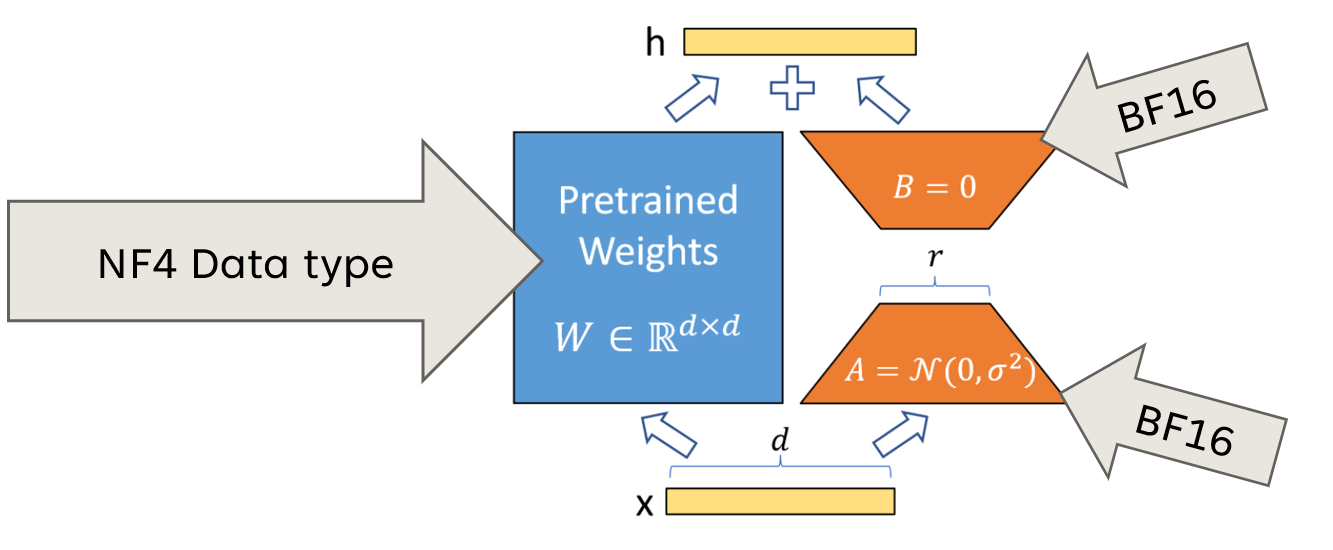
\includegraphics[width=\linewidth]{img/qlora.png}
    \caption{Model parameters under QLoRA NF4 + LoRA: frozen backbone in 4-bit quantization with per-channel scales; trainable LoRA parameters in higher precision; forward/backward compute in bf16.}
    \label{fig:qlora}
\end{figure}

\section{Tokenization}
Tokenization converts raw text into a sequence of discrete token IDs drawn from a fixed vocabulary. Language models as one of the first forward pass steps consume sequence of token IDs as input and map them to their embeddings vectors. A good scheme balances coverage (few unknowns), compact sequences (shorter length for a given text), and stability of encoding/decoding.

\subsection{Subword methods}
Pure word-level vocabularies suffer from out-of-vocabulary (OOV) issues, while character-level tokenization produces very long sequences. Subword tokenization offers a compromise by decomposing words into frequent subunits that compose to any string, including rare words and misspellings \cite{sennrich2016neuralmachinetranslationrare}.

Common approaches:
\begin{itemize}
    \item \textbf{Byte-Pair Encoding (BPE)}: the most widely used method in modern LLMs, starts from a large text corpus and iteratively merges the most frequent adjacent pairs to form larger subwords until a target vocabulary size is reached \cite{sennrich2016neuralmachinetranslationrare}. BPE yields deterministic segmentations given the learned merges and has no explicit probabilistic model.
    \item \textbf{WordPiece}: subword units to maximize likelihood of a training corpus, typically under a simple probabilistic model over segmentations; greedy decoding selects the best segmentation. It typically includes reserved continuation markers to indicate that a subword is not word-initial.
    \item \textbf{SentencePiece}: optimizes a probabilistic unigram model over a candidate subword inventory and prunes units that hurt likelihood \cite{kudo2018sentencepiecesimplelanguageindependent}. It supports sampling alternative segmentations during training for robustness and can operate directly on raw text without external pre-tokenization.
\end{itemize}

Implementation frameworks such as SentencePiece and Transformers provide standardized training, encoding, and decoding pipelines \cite{kudo2018sentencepiecesimplelanguageindependent,wolf2020huggingfacestransformersstateoftheartnatural}. Variants like byte-level BPE ensure coverage of arbitrary Unicode by operating on UTF-8 bytes, which removes true OOVs at the cost of sometimes longer sequences for non-Latin scripts.

\begin{figure}[t]
    \centering
    \includegraphics[width=\linewidth]{figures/tokenization-examples.pdf}
    \caption{Tokenization }
    \label{fig:tokenization-examples}
\end{figure}

\subsubsection{Vocabulary}
Larger token vocabularies can represent up to whole words, reducing sequence length and attention cost. However, they implicitly increase embedding and output layer sizes, memory, and may cause overfitting. Smaller vocabularies generalize better to rare forms but inflate sequence length, which increases quadratic attention cost and risk of truncation. Practical choices range from 16k-200k subwords.

\subsubsection{Normalization and pre-tokenization.}
Many pipelines normalize text (e.g., Unicode NFKC, lowercasing, whitespace handling) to improve robustness; SentencePiece can integrate normalization and avoid external word boundary rules \cite{kudo2018sentencepiecesimplelanguageindependent}. Pre-tokenizers may split on whitespace and punctuation to enforce word boundary awareness before applying subword merges. Choices here affect how punctuation, casing, and whitespace survive round-trip detokenization.

\subsection{Special tokens and sequence framing}
Special tokens mark structure and control decoding:
\begin{itemize}
    \item \textbf{BOS/EOS}: Begin-of-sequence and end-of-sequence delimit the sequence and signal termination.
    \item \textbf{PAD}: Padding aligns sequences within a batch to a common length; attention masks ensure pads are ignored during loss computation and attention.
    \item \textbf{Instruction tokens}: Special markers that indicate task boundaries or specify desired behavior (e.g., \texttt{<|user|>}, \texttt{<|assistant|>}, \texttt{<|thought|>}).
\end{itemize}
Figure~\ref{fig:sequence-framing} shows the instruction/assistant turn framing and BOS/EOS/PAD usage.

\begin{figure}[t]
    \centering
    \includegraphics[width=\linewidth]{figures/sequence-framing.pdf}
    \caption{Sequence framing with special tokens: example instruction–response turns using BOS/EOS and task-specific role tokens (e.g., <|user|>, <|assistant|>).}
    \label{fig:sequence-framing}
\end{figure}

\section{GSM8K}
GSM8K is a benchmark of 8.5K English grade-school math word problems designed to evaluate multi-step reasoning in natural language \cite{cobbe2021trainingverifierssolvemath}. Problems typically require 2-8 steps of elementary arithmetic ($+,-,\times,\div$) and include human-written, natural-language solutions with inline ``calculator annotations'' (intermediate computations) and a final integer answer on a separate line. The benchmark is widely used to study prompting and reasoning supervision; standard scoring is exact numeric match, often evaluated under chain-of-thought prompting and self-consistency sampling \cite{wei2023chainofthoughtpromptingelicitsreasoning,wang2023selfconsistencyimproveschainthought}.

\subsection{Dataset overview and structure}
Released in English via HuggingFace Datasets \cite{lhoest2021datasetscommunitylibrarynatural}, GSM8K provides two configurations: a main set (question, rationale, final answer) and a socratic variant that interleaves sub-questions within the solution. Official splits comprise 7{,}473 training and 1{,}319 test problems \cite{cobbe2021trainingverifierssolvemath}; each instance pairs a question string with a multi-step natural-language solution containing intermediate calculations and a single integer final answer.
Figure~\ref{fig:gsm8k-example} shows an example question, rationale with inline calculations, and final integer answer line.

\begin{figure}[t]
    \centering
    \includegraphics[width=\linewidth]{figures/gsm8k-example.pdf}
    \caption{GSM8K example: (left) problem statement; (right) step-by-step rationale with calculator-style intermediate computations, followed by a final integer answer on its own line.}
    \label{fig:gsm8k-example}
\end{figure}